\section{Text-Driven Video Editing: Text2LIVE}
\begin{frame}[allowframebreaks]{Text2LIVE}
    \textbf{Text2LIVE} (Bar-Tal et al., ECCV 2022) edits \emph{existing} images and videos from a text prompt: instead of generating a video from scratch, it changes the appearance of objects or adds semi-transparent effects while keeping the rest of the footage intact.

    \begin{itemize}
        \item \textbf{Layered editing:} the edit is generated on a separate RGBA layer that is composited over the original frames, so the source content is preserved.
        \item \textbf{Neural atlases:} the video is decomposed into 2D atlases (foreground/background); editing the atlas propagates the change consistently across all frames.
        \item \textbf{CLIP supervision, zero-shot:} the edit layer is optimized so the result matches the text prompt under CLIP similarity; no paired training data; instead a generator is trained per input (internal learning) at test time.
        \item \textbf{Contrast with generation:} complements the text-to-video simulators seen earlier; here language steers \emph{modification} of real footage rather than synthesis from noise.
    \end{itemize}
\framebreak
    \begin{figure}
        \centering
        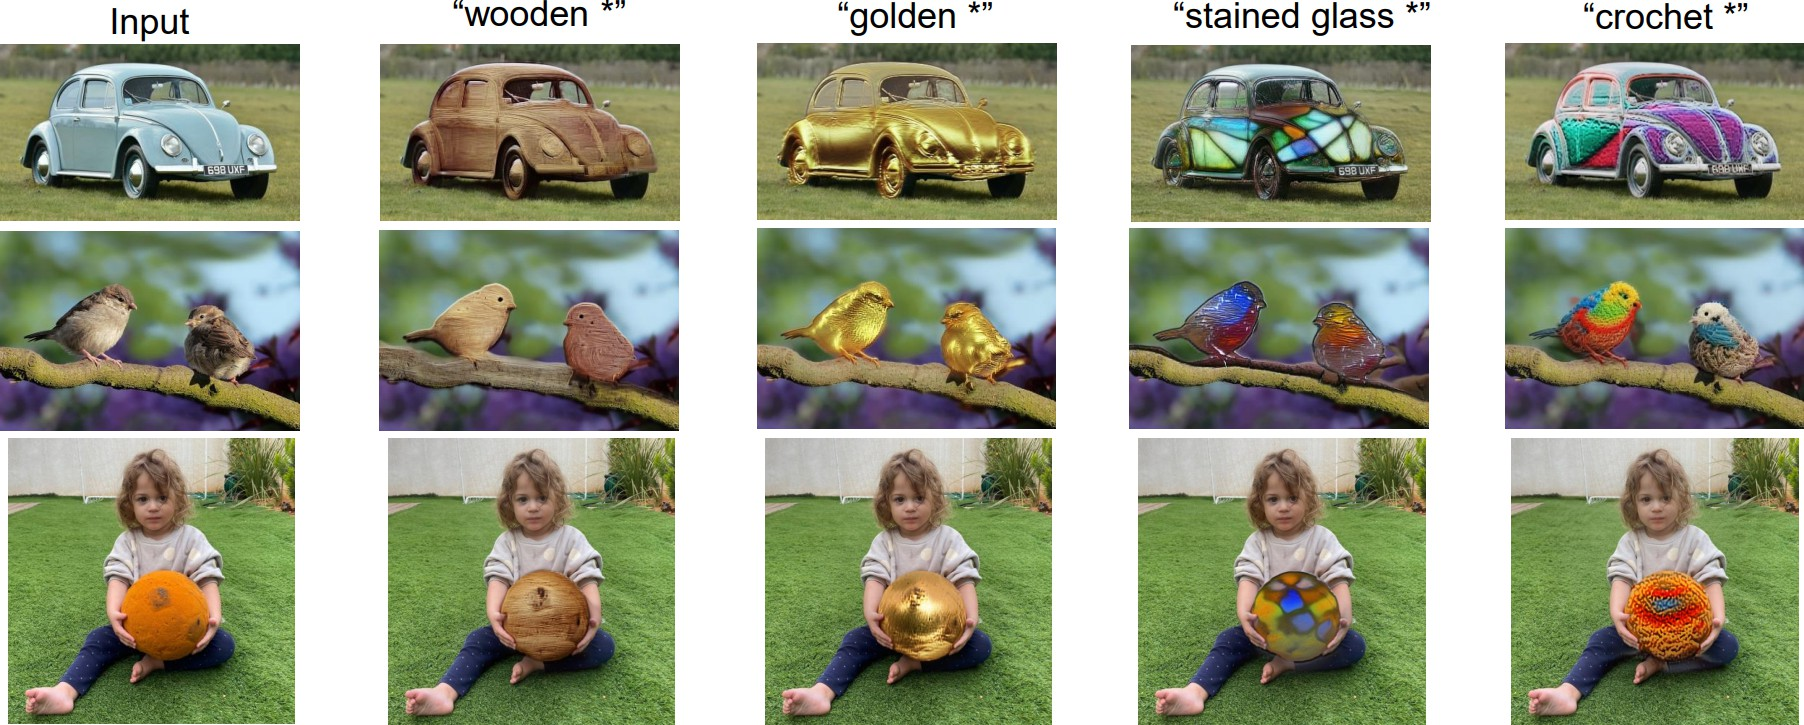
\includegraphics[width=1\textwidth,height=0.8\textheight,keepaspectratio]{images/video-generation/text2live_layered_editing_examples.jpg}
    \end{figure}
    {\footnotesize{[Text2LIVE: Text-Driven Layered Image and Video Editing, Bar-Tal, Ofri-Amar, Fridman, Kasten \& Dekel, ECCV 2022]}}
\end{frame}
